\title{Peer Review 1 for Yinan}
\author{
        Spencer Woody \\
                SDS 383D
}
\date{\today}

\documentclass[11pt]{article}

\usepackage{graphicx}
\usepackage{amsmath}
\usepackage{listings}
\usepackage{hyperref}
\hypersetup{
    colorlinks = true%,
%    linkbordercolor = {white}
}
\usepackage[]{algorithm2e}
\usepackage{mathpazo}
\usepackage{inconsolata}

\begin{document}

\maketitle

\setlength{\parindent}{0cm}

\section{Introduction}

Hi Yinan, I enjoyed reviewing your problem set and code. It looks like you understand the topics very well. Still, I have a few pieces of feedback to give for you to improve your \LaTeX and \textsf{R}, and create good write-ups for these exercises in the future.

\section{General notation tips}

\subsection{Vectors}

It is best to \emph{not} use the notation $\vec{x}$ to denote a vector because it is easy to confuse this with the sample mean, $\bar{x} = \sum_{i=1}^n x_i / n$. Instead, you can use a bold-faced $\mathbf{x}$ or simply $x$, and then the scalar components are referenced with subscripts, e.g. $x_i$. I will post the \texttt{.tex} file I used to make this report on my Github so that you can see how I produced all of these. 

\subsection{Proportionality sign, $\propto$}

It looks like in most of your write-up, you used the full version of Bayes' Theorem, i.e.,
%
\begin{align*}
	p(\theta | x) &= \frac{p(x|\theta)p(\theta)}{\int_\Theta p(x|\theta)p(\theta) d\theta}.
\end{align*}
%
While this form is very explicit, it is both convenient and more legible to write this as 
%
\begin{align*}
	p(\theta | x) &\propto p(x|\theta)p(\theta)
\end{align*} 
%
where the $\propto$ symbol is produced with the command \begin{verbatim}
	\propto
\end{verbatim}
%
and, furthermore, this is helpful in writing PDFs. For instance, If $X\sim \text{Ga}(\alpha, \beta)$, the the PDF of $X$ may be written in terms of proportionality 
%
\begin{align*}
	p_X(x) &\propto x^{\alpha - 1} \exp \left(-\beta x \right).
\end{align*}
% 
This way, it is easier to derive the kernels of whatever posterior distributions without the cluttering of the proportionality constants, which are really only there to ensure the PDF integrates to 1.

\subsection{$\exp$ vs. $e$}

If you are writing a long exponential term, it is better to represent it as $\exp(\bullet)$ rather than $e^\bullet$. For instance, $$\exp \left[ -\frac{1}{2}(y - X\beta)^T \Sigma(y - X\beta) \right]$$ is much easier to read than $$ e^{-\frac{1}{2}(y - X\beta)^T \Sigma(y - X\beta)} .$$ In fact, I rarely ever use $e^\bullet$ just to keep my writing as consistent and legible as possible. Within math environments, the command to produce an upright $\exp$ is very simple: \begin{verbatim}
	\exp
\end{verbatim}

\subsection{Using \texttt{\textbackslash left} and \texttt{\textbackslash right}}

On a related note, if you are trying to put parentheses or brackets around a ``tall'' expression, if it is advantageous to use the commands \texttt{\textbackslash left} and \texttt{\textbackslash right}. For instance, \begin{verbatim}
	\exp \left[ -\frac{1}{2}(y - X\beta)^T \Omega(y - X\beta) \right]
\end{verbatim}
%
produces $$ \exp \left[ -\frac{1}{2}(y - X\beta)^T \Omega(y - X\beta) \right] $$ while \begin{verbatim}
	\exp [ -\frac{1}{2}(y - X\beta)^T \Omega(y - X\beta) ]
\end{verbatim}
%
produces $$ \exp [ -\frac{1}{2}(y - X\beta)^T \Omega(y - X\beta) ]. $$ You can see that in the latter case, the brackets do not encolse the entire expression in the exponential function. 

\section{Giving context in your writing}

When I was reading through your write-up, I had trouble remembering what question was originally asked in the problem set for any given section. Your typeset equations generally look very good, but do be sure to give some background in each section of your write-up dedicated to explaining what's going on. And also give some rationale for what you are doing, or give sources for where you got your information. For example, in your MLE section you give the MLEs for the mean vector and covariance matrix without any derivation. And you also gave the results of inverting the covariance matrix without deriving that either. Including this information would make your report easier to follow, not only for outside audiences but also for yourself when you want to return to read it later. 

\section{The Bootstrap}

If I remember correctly, you made a presentation on the bootstrap for the MLE of the mean vector and covariance matrix of the multivariate. I thought it was interesting that you showed the \emph{actual} sampling distribution of the MLEs (normal for the mean vector, Wishart for the covariance matrix). However, the entire point of the bootstrap is to \emph{approximate} these sorts of sampling distributions by using Monte Carlo resampling with replacement from the empirical distribution. So what I did for my bootstrap was to just do approximately 10,000 resamples, and each time compute the MLEs and store them to a matrix. From this you can make a histogram of each component. For example, the first figure below shows the sampling distribution of each element of the mean vector, and the second figure shows the sampling distribution of each element in the covariance matrix, with the dashed blue line representing the median of Monte Carlo estimates, and the red solid line representing the true value. 
\pagebreak

\begin{figure}[htp!]
	\centering
		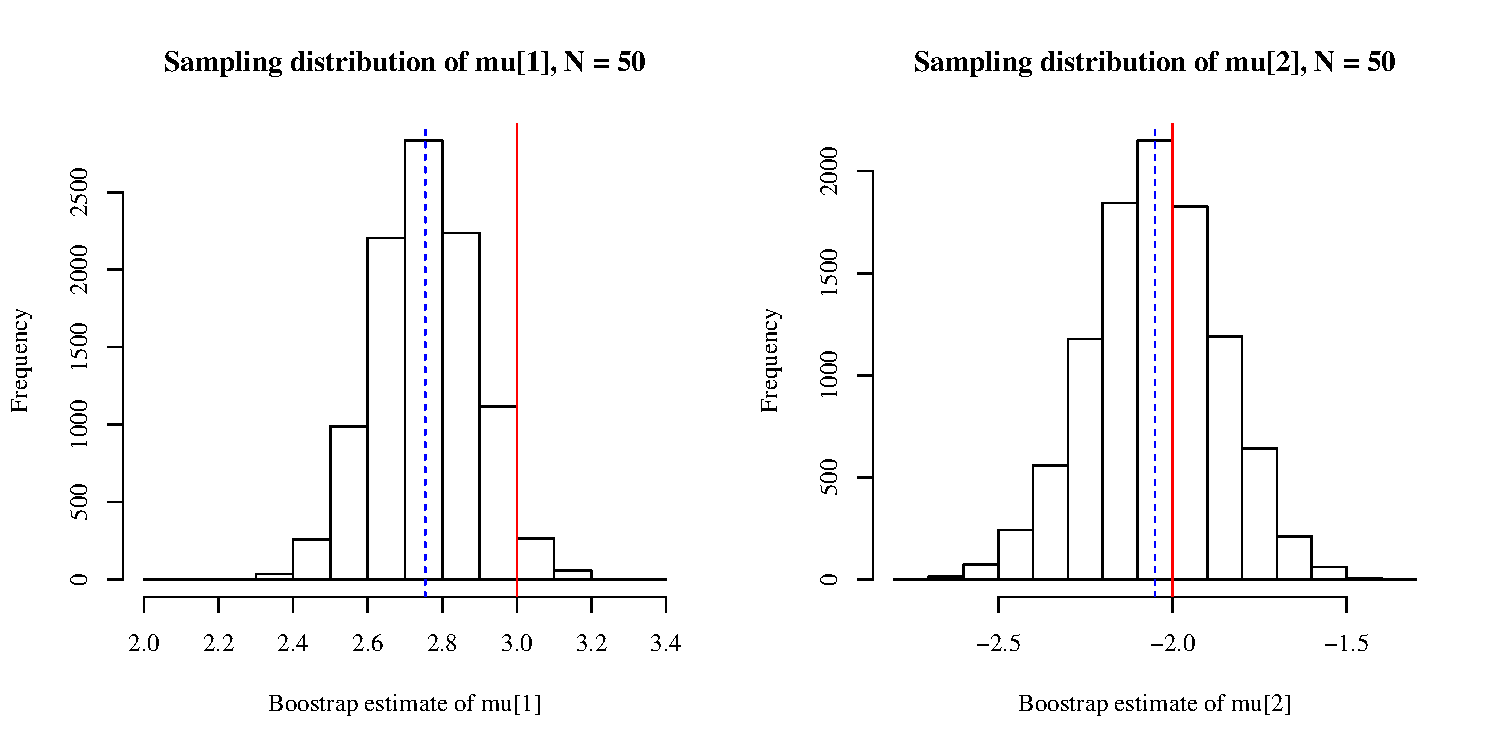
\includegraphics[scale=0.6]{mu.pdf}
	\caption{Bootstrap estimate of the sampling distribution of MLE of mean vector from a sample of mutivariate normal variables}
\end{figure}

\pagebreak

\begin{figure}[htp!]
	\centering
		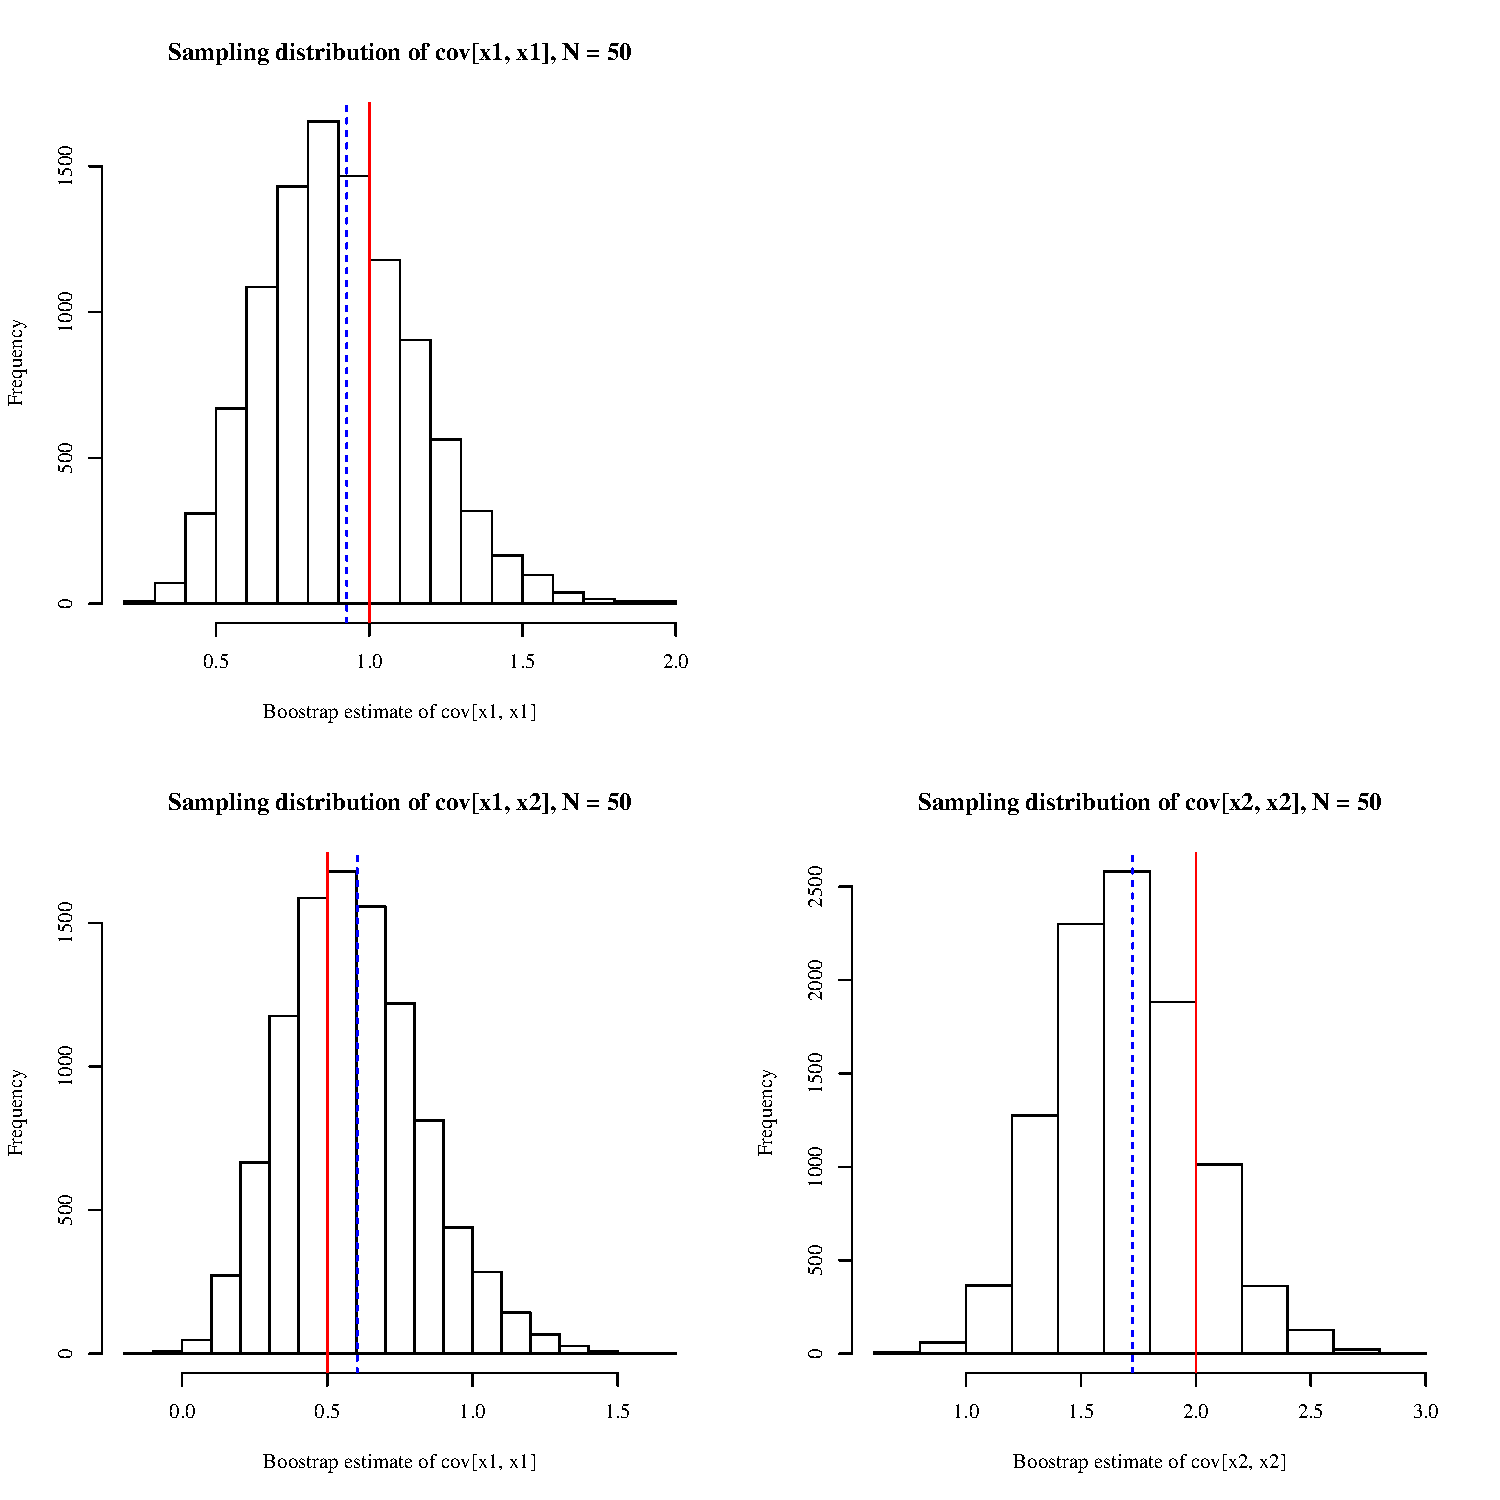
\includegraphics[scale=0.6]{Sigma.pdf}
	\caption{Bootstrap estimate of the sampling distribution of MLE of covariance matrix from a sample of mutivariate normal variables}
\end{figure}

\pagebreak

I encourage you to read Bradley Efron's original 1979 paper published in \emph{The Annals of Statistics} titled ``Bootstrap Methods: Another Look at the Jackknife'' (available online \href{http://www.stat.cmu.edu/~fienberg/Statistics36-756/Efron1979.pdf}{here}) and I also made a slideshow presentation about this paper which you can find on my \href{https://github.com/spencerwoody/SDS190/blob/master/Spencer_slideshow.pdf}{Github}. Efron defines the concept of the bootstrap so generally that once you learn his notation and approach, it is easy to apply this principle to many difference circumstances. 

\section{\textsf{R} Code}

Your \textsf{R} code was pretty straightforward, and I don't have too much to add to it. However, I noticed a few things you can do to streamline it. It is best to follow some sort of style guide. My personal favorite comes from \href{https://google.github.io/styleguide/Rguide.xml}{Google}, but it's really all about making your code as readable as possible to someone who has never seen your problem before. My biggest pieces of advice in terms of notation would be 1) use \texttt{<-} for assigning variables rather than an equal sign (which should only be used for logical statements and arguments in functions), and 2) use some sort of clever system of comments in your code to separate sections into easily distinguishable chunks.

\subsection{Matrix algebra (multiplying and inverting)}

Matrix math in \textsf{R} can be somewhat clunky, and there are a few tricks that I think everything should learn. \texttt{crossprod} is fast for inner products, \texttt{tcrossprod} is fast for outer products, and \texttt{solve(A, b)} is much more stable than \texttt{solve(A) \%*\% b} for computing $A^{-1}b$. Check out the \href{https://cran.r-project.org/web/packages/Matrix/index.html}{Matrix} package for more on cutting down on computational costs.

\section{Conclusion}

Overall, great job with this first assignment. I found your write-up mostly easy to follow. I hope this review has been helpful for you, and do not hesitate to ask me to clarify anything or give any other tips. \\

Spencer

\end{document}

